\section{Data and Measurement}\label{sec:data_and_measu}

The data used for this paper are drawn from the publicly available replication package for \cite{hengel2022publishing}, hosted on GitHub. The data package covers 11695 English-language articles from the years 1950 to 2015 from 5 top journals in economics: American Economic Review (AER), Quarterly Journal of Economics (QJE), Econometrica (ECMA), Review of Economic Studies (ReSTUD), and Journal of Political Economy (JPE). The majority of the analysis in this paper excludes ReSTUD, which \cite{hengel2022publishing} includes primarily for its availability of submission-acceptance dates, and AER Papers \& Proceedings, which do not contain abstracts. A full breakdown of articles by journal and decade is in Appendix~\ref{sec:Summary Statistics}.  

The article data includes the title, abstract, citation count, submission and acceptance date, JEL codes, and pre-computed readability scores from \cite{hengel2022publishing}. The article data is linked with author-level data on gender, native language, and institution. 

For this paper, we do not re-estimate readability scores or re-verify the gender coding of \cite{hengel2022publishing}. We also exclude any analysis of full-text readability, as processing the full text through the LLM would be prohibitively expensive at scale and because evaluation quality degrades with longer inputs (\cite{modarressi2025nolimalongcontextevaluationliteral}). 

Following \cite{hengel2022publishing}, our main specification classifies papers as 'male-authored' when women constitute a strict minority of the author team. For papers where women are a majority, the gender variable is defined as the ratio of female to male authors. 

\begin{figure}[H]
    \centering
    \begin{subfigure}{0.48\textwidth}
        \centering
        
\includegraphics[width=\textwidth]{figures/Figure-1.pdf}
        \caption{Flesch Readability}
        \label{fig:panel_a}
    \end{subfigure}
    \hfill
    \begin{subfigure}{0.48\textwidth}
        \centering
        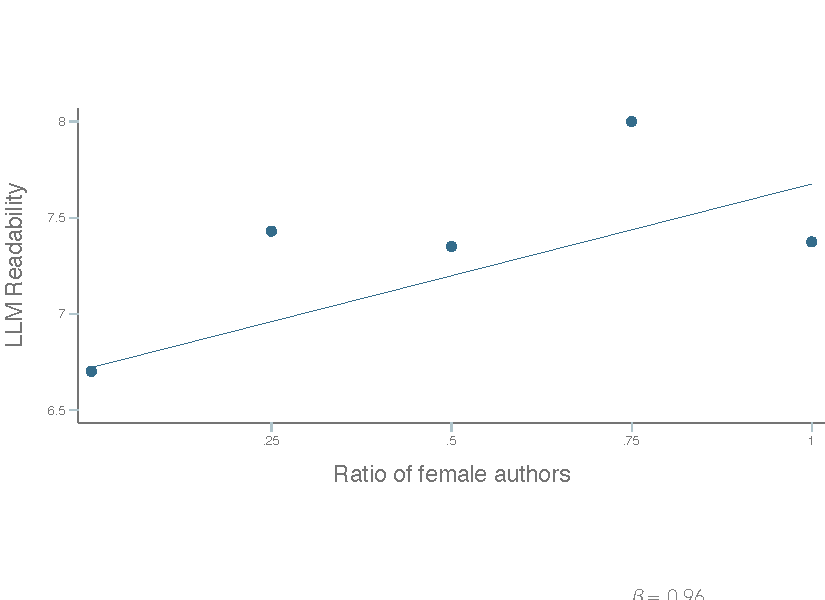
\includegraphics[width=\textwidth]{figures/Figure-1-llm.pdf}
        \caption{LLM Readability}
        \label{fig:panel_b}
    \end{subfigure}
    \caption{Relationship between readability and the ratio of female authors}
    \label{fig:both_panels}
\end{figure}

Figure~\ref{fig:both_panels} plots readability against the female author ratio for two measures: Flesch readability (copied from \cite{hengel2022publishing}) and LLM readability. Although they both show a broadly positive relationship, they differ in shape. For robustness, we therefore also estimate our main results under alternative authorship specifications: 
\begin{itemize}
  \item Using a binary equal to 1 if the article's authors are majority female
  \item Using a binary equal to 1 if there is 1 female coauthor
  \item Using only single-gender papers
  \item Using only solo-authored articles
  \item Comparing articles with a senior female coauthor to entirely male-authored papers
\end{itemize}

Further description of the data can be found in Section 2 and Appendices C and D of \cite{hengel2022publishing}.

\subsection{Tonal Analysis Rubric}\label{sec:Rubric}

Additionally, we use a 16-item rubric to evaluate paper abstracts on the scale of 1-10 for Modal Verb Strength, Hedging Frequency and Type, Qualifier Density, Acknowledgment of Limitations, Caution-Signaling Connectors, Assertiveness and Voice, Active/Passive Voice Ratio, Sentence Length and Directness, Imperative-Form Occurrence, Pronoun Commitment, Novelty-Claim Strength, Jargon and Technicality Density, Emotional Valence, Evidence and Citation Usage, Practical and Impact Orientation, Readability. See exact evaluation rubric in Appendix: \nameref{sec:rubric}.

\subsection{LLM Evaluations}\label{sec:LLM_Evaluations}

To conduct the tonal evaluations, we developed a Large Language Model (LLM) powered algorithm that would take the abstracts from the papers, process them into a readable LLM message, and then pass the message through to the LLM, which would, in turn, provide a structured output of evaluations. The LLM model we chose for this analysis was GPT-5, which includes both standard LLM capabilities and the ability for more complex reasoning. We valued the model’s ability to generate detailed thinking processes before answering to handle the complexity of our multi-dimensional tonal analysis rubric, as reasoning models have performed better than non-reasoning models as task complexity increases (\cite{shojaee2025illusionthinkingunderstandingstrengths}). This also allowed us to keep our input token count to a minimum, which increases model accuracy (\cite{modarressi2025nolimalongcontextevaluationliteral}). 

This process of passing the abstracts and rubric to the model is sufficient to generate the needed evaluations, but insufficient in providing the most accurate responses. To increase response accuracy, we implemented prompt engineering, a process of creating clear instructions for the model to increase performance (\cite{openai_prompt_engineering}). Part of this process is to induce step-by-step thinking in the model and allow for model reasoning for each section of the rubric, both shown to increase model accuracy (\cite{zhang2022automaticchainthoughtprompting}).

To validate the accuracy of the evaluations, we first trained the algorithm on a small subset of abstracts, auditing the evaluation output and reasoning for these responses and using that to improve our prompt. We then tested the algorithm on a different subset of abstracts to validate the output and reasoning before running the algorithm on the full dataset. A separate validation was performed using readability scores, comparing our outputs against \textcite{hengel2022publishing} manually calculated readability scores, checking to see if our evaluations were consistent with hers at the population level. 

Despite the validation involved with calibrating the LLM for our project, there is still some randomness involved in the LLM evaluations. Because of this, the standard errors for analysis using LLM evaluations do not fully reflect the instability of our estimates.